\documentclass[sigconf,natbib=false,10pt]{acmart}
\settopmatter{printacmref=false}
\setcopyright{none}
\renewcommand\footnotetextcopyrightpermission[1]{}

\acmConference[SOSP '24]{Workshop on Hot Topics in Operating Systems}{November
2024}{Austin, TX, USA}

%\begin{CCSXML}
%<ccs2012>
%   <concept>
%       <concept_id>10002978.10003029.10011703</concept_id>
%       <concept_desc>Security and privacy~Usability in security and privacy</concept_desc>
%       <concept_significance>300</concept_significance>
%       </concept>
%   <concept>
%       <concept_id>10002951.10002952.10003190</concept_id>
%       <concept_desc>Information systems~Database management system engines</concept_desc>
%%       <concept_significance>300</concept_significance>
%       </concept>
% </ccs2012>
%\end{CCSXML}

%\ccsdesc[300]{Security and privacy~Usability in security and privacy}
%\ccsdesc[300]{Information systems~Database management system engines}

% to be able to draw some self-contained figs
\usepackage{tikz}
\usepackage{amsmath}
\usepackage{hyperref}
\usepackage[normalem]{ulem}
\usepackage{listings}
\usepackage{xspace}
\usepackage{booktabs}
\usepackage{multirow}
\usepackage{wasysym}
\usepackage{caption}
\usepackage{subcaption}
\usepackage{enumitem}
\usepackage[utf8]{inputenc}
\usepackage[compact, small]{titlesec}

\captionsetup{labelfont=bf,textfont=rm,belowskip=-8pt,aboveskip=4pt}

% BibLaTeX for bibliography
\usepackage[
  backend=biber,
  style=numeric-comp,
  minalphanames=3,
  isbn=false,
  sortcites=true,
  sorting=anyt,
  abbreviate=false,
  url=false,
  doi=false,
  maxnames=99,
  minbibnames=3,
  maxbibnames=99]{biblatex}
\addbibresource{paper.bib}

\AtBeginBibliography{\small}
\setcounter{biburllcpenalty}{7000}
\setcounter{biburlucpenalty}{8000}

\newcommand\sysname{Cole}

\newcommand\hmng[1]{\textcolor{blue!40!red}{[hmng: {#1}]}}
\newcommand{\tabitem}{~~\llap{\textbullet}~~}
\newcommand{\eg}{{e.g.},\xspace}
\newcommand{\ie}{{i.e.},\xspace}

\newcommand{\one}{({\em i}\/)}
\newcommand{\two}{({\em ii}\/)}
\newcommand{\three}{({\em iii}\/)}
\newcommand{\four}{({\em iv}\/)}
\newcommand{\five}{({\em v}\/)}
\newcommand{\six}{({\em vi}\/)}



\lstdefinestyle{rust}{
    %backgroundcolor=\color{backcolour},
    commentstyle=\color{codegreen},
    keywordstyle=\color{codepurple},
    stringstyle=\color{blue},
    basicstyle=\ttfamily\scriptsize,
    breakatwhitespace=false,
    breaklines=true,
    captionpos=b,
    keepspaces=true,
    showspaces=false,
    showstringspaces=false,
    showtabs=false,
    tabsize=2
}
\lstset{style=rust}

%-------------------------------------------------------------------------------
\begin{document}
%-------------------------------------------------------------------------------

%don't want date printed
\date{}

%%
%% The "title" command has an optional parameter,
%% allowing the author to define a "short title" to be used in page headers.
% make title bold and 14 pt font (Latex default is non-bold, 16 pt)
\title{Don't get SLAmmed: know your deadlines}

%%
%% The "author" command and its associated commands are used to define
%% the authors and their affiliations.
%% Of note is the shared affiliation of the first two authors, and the
%% "authornote" and "authornotemark" commands
%% used to denote shared contribution to the research.

% \author{
% {\rm Anonymous Authors}\\
% } % end author

\author{Hannah Gross}
\affiliation{%
 \institution{MIT}
 \state{Graduate Student}
  \country{}
}

\author{Frans Kaashoek}
\affiliation{%
 \institution{MIT}
 \state{}
  \country{}
}

\maketitle

%-------------------------------------------------------------------------------
\section{Introduction}
\label{s:intro}
%-------------------------------------------------------------------------------

Cloud providers like AWS and Google, as well as deployment management systems
like Kubernetes, allow users to run services by attaching to each an amount of
resources the service will get. This includes compute (a number of vCPUs),
memory, and sometimes network bandwidth~\cite{aws-ec2-resources,
kubernetes-resources}; the resource this work focuses on is CPU. The guarantee
developers get is that the service will have undisturbed access to that amount
of resources.

Enforcing this guanatee is hard. If providers leave the CPUs idle so they are
available when the service needs them, that leads to a utilization problem. The
load on most applications run in the cloud is variable and unpredictable, so to
account for this developers choose the amount of resources to reserve based on
the expected peak load~\cite{borg, nu, overprovision}. This means that services
with reserved resources rarely use the full reservation they asked for. 

What most systems do instead is allow other workloads to run opportunistically
on temporarly unutilized resources. This includes so-called \textit{best effort}
workloads, which have no reservations, as well letting services with
reservations temporarily \textit{burst}, meaning use more CPUs than they asked
for. This solves the utilization problem, without requiring compromises on the
guarantees made: services with reservations get access to the CPUs they
requested when desired, while best effort or bursting services can make use of
otherwise idle resources.

Kubernetes follows presicely this model. Services fall into three quality of
service (QOS) classes: \textit{Guaranteed}, which have requests (\ie{}
reservations) as well as limits, \textit{Burstable}, which have requests and no
limits, and \textit{Best Effort}, which have
neither~\cite{kubernetes-pod-qos-types}. Guaranteed services are the last to be
evicted from a node experiencing high load, and give more predictable
performance, whereas the Burstable class allows applications with bursty load to
opportunistically make use of available resources, thereby better utilizing the
resources Kubernetes is running on.

AWS similarly supports both guaranteed- and burstable-style reservations, with
their M and T instance types~\cite{aws-ec2-burstable,aws-ec2-resources}. In this
case the motivation for customers to use the burstable-style instance rather
than overprovisioning on guaranteed-style is pricing.


\begin{figure}[t]
    \centering
    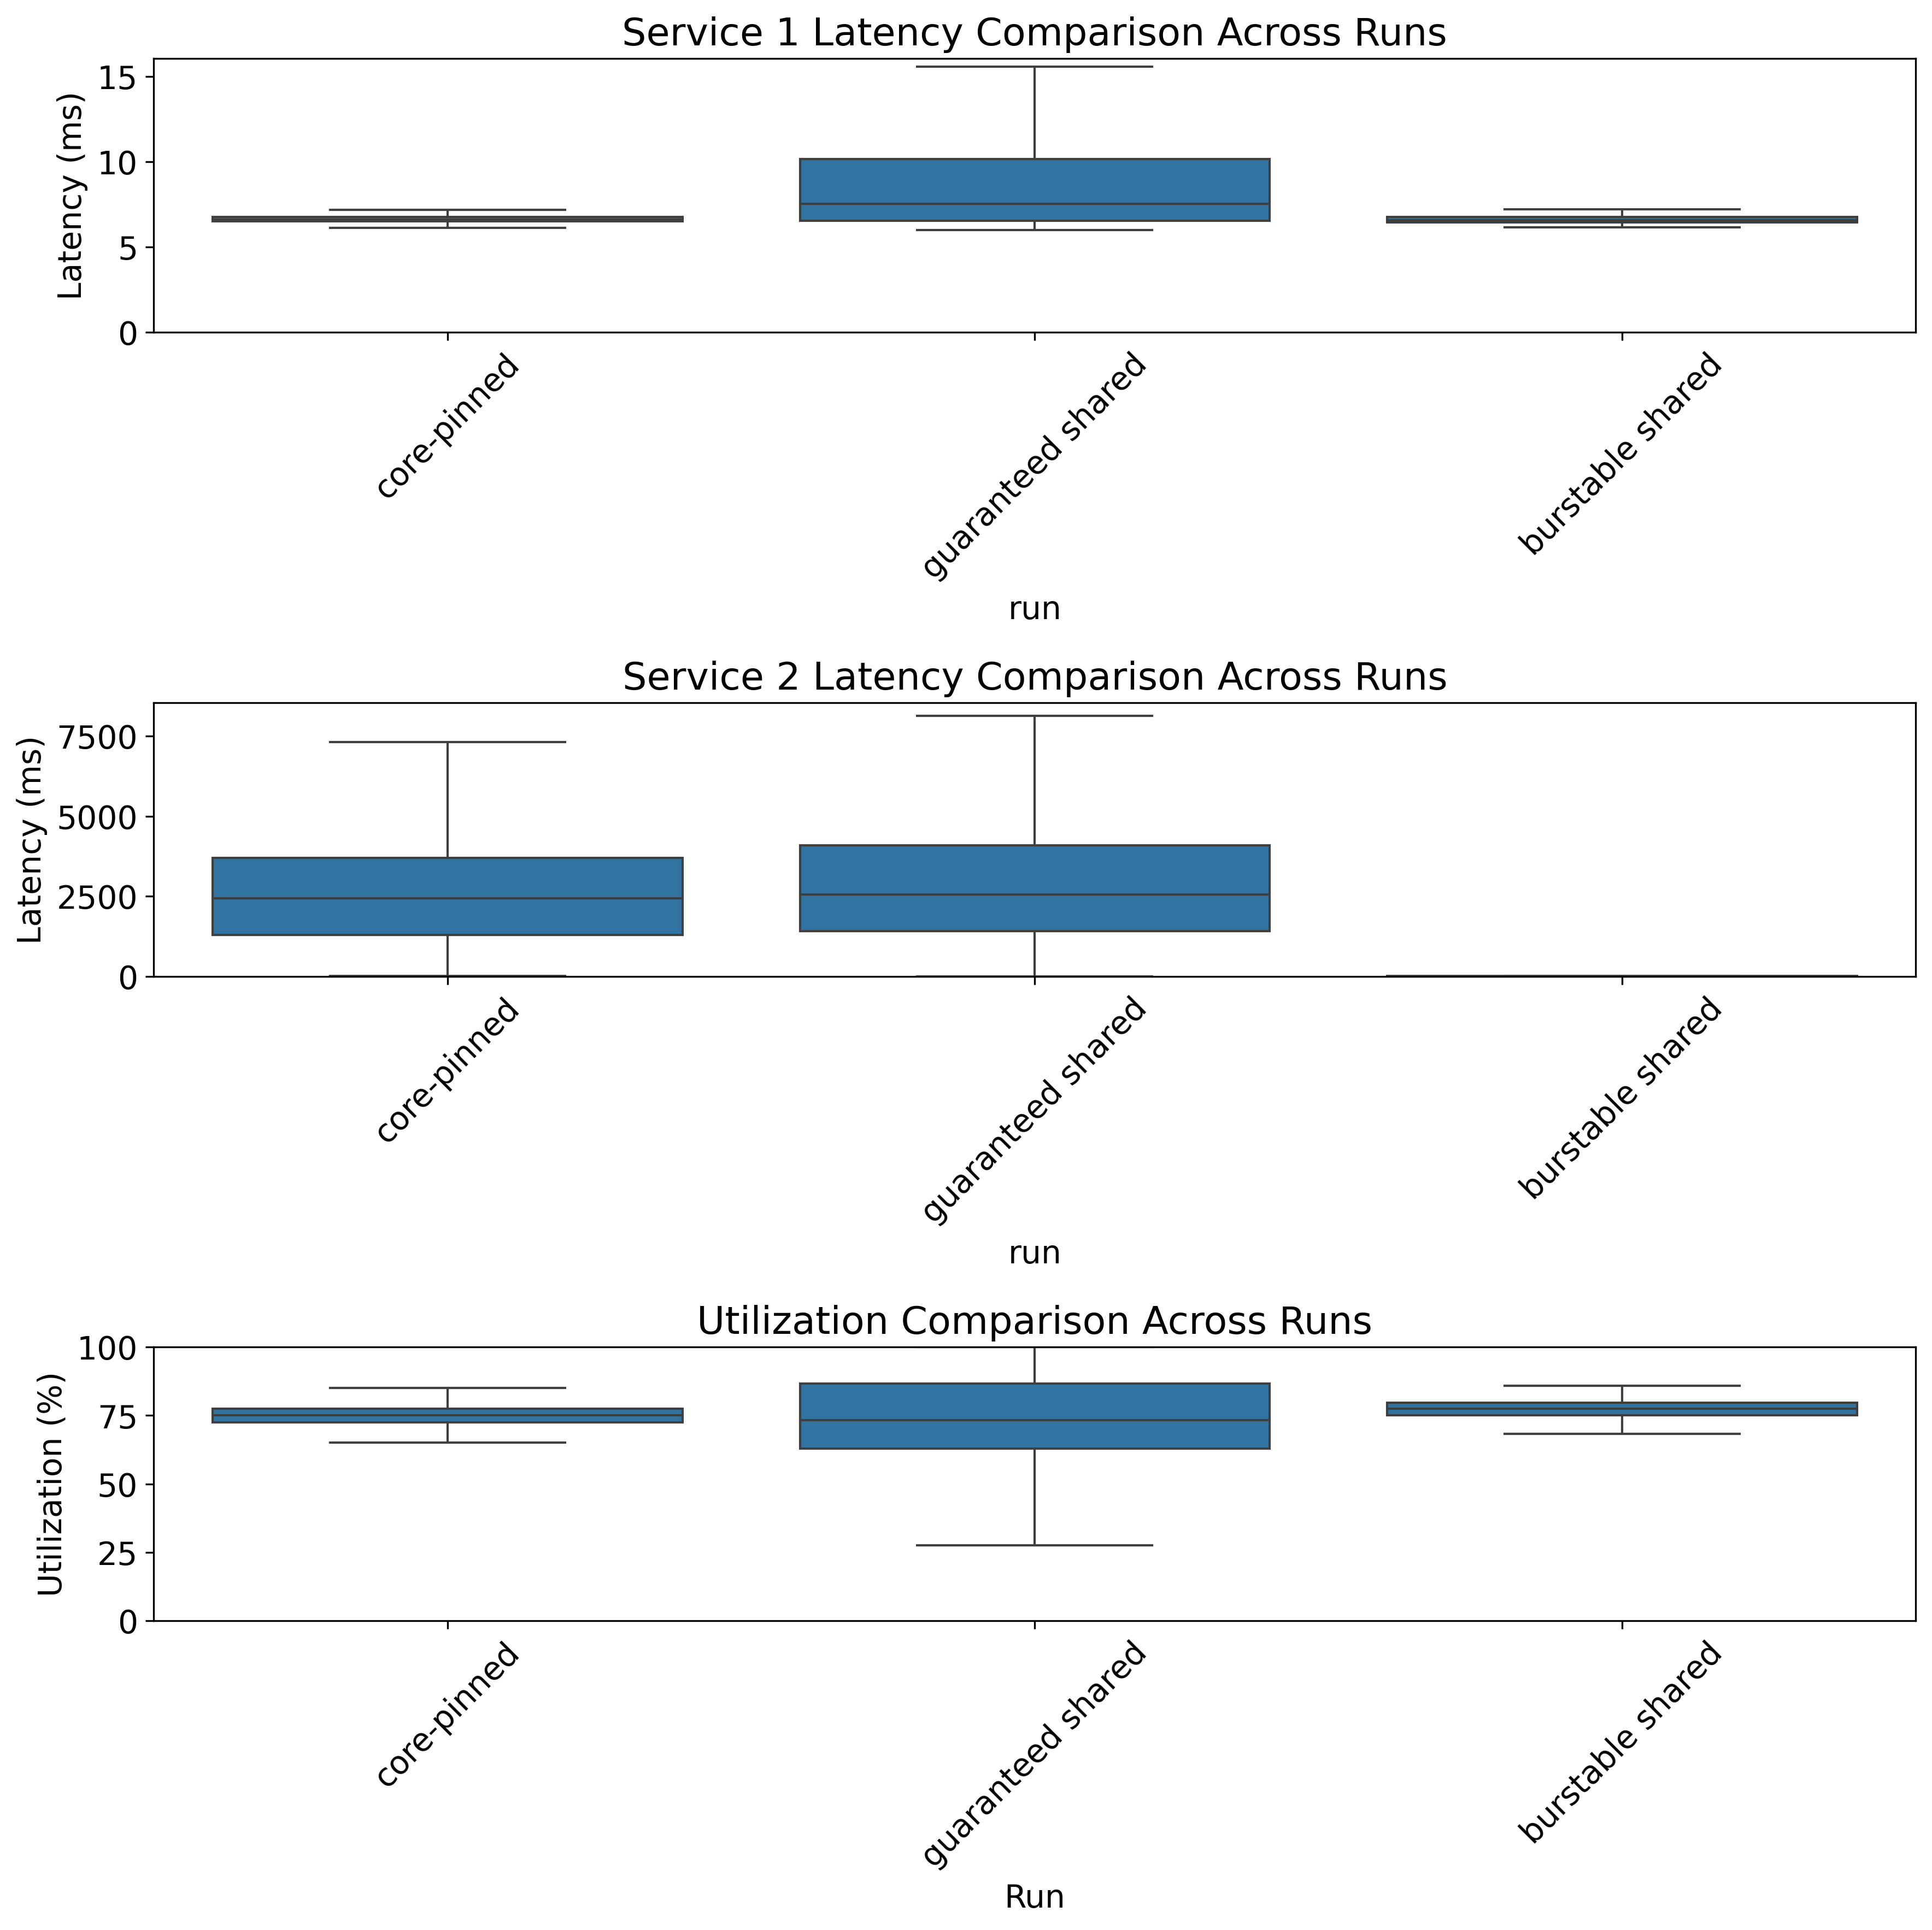
\includegraphics[width=\columnwidth]{graphs/kubernetes-lc-lc-cmp.png}
    \caption{In Kubernetes, running anything alongside a server in the
    Guaranteed QOS class affects the server's
    performance}\label{fig:kubernetes-qos-cmp}
\end{figure}

However, we find that current popular scheduling systems fail to properly
enforce reservations. We use as a case study a small but realistic social
network web application, which we run using Kubernetes.
\autoref{fig:kubernetes-qos-cmp} shows that running anything, even another
guaranteed service, alongside the web server affected its end-to-end latencies,
and that these effects go away when using core-pinning.\hmng{edited up to here}

Understanding why Kubernetes fails to honor the web application's reservation
requires looking at the underlying mechanism enforcing the CPU reservation:
Linux's \cgroups{}. In fact, most modern containers rely on \cgroups{} for CPU
isolation: all Open Container Initiative (OCI) compliant containers, including
Kubernetes but also Docker, CRI-O, and containerd
do~\cite{oci-cgroups,docker-docs-cgroups,container-isolation-article}. VM
frameworks, including Firecracker, AFaas and libvirt, also rely on \cgroups{} to
manage CPU time reservation~\cite{firecracker-cgroups,afaas,libvirt-cgroups}.

Weight is the part of the \cgroups{} interface these systems use for enforcing
the reservations LC applications have, while still allowing BEs without
reservations to run opportunistically.\footnote{Other operating systems expose a
similar interface, for instance Windows exposes a number of shares.} Kubernetes
creates one top level group for all best effort services, called
\texttt{kubepods-besteffort}, inside which all BE pods are placed, and assigns
it the lowest possible weight of 1. Pods with reservations are separated into
Burstable and Guaranteed, the main difference being that Guaranteed pods require
a limit to be set on the resources it can use. Kubernetes calculates the weight
that each pod gets based on the amount of milliCPUs it requests. For instance,
in the \autoref{fig:kubernetes-unedited} experiment, the web application service
ran in the Guaranteed class and asked for 4 CPUs, and Kubernetes assigned the
underlying pod a weight of 157.

The \cgroups{} documentation specifies that each group should get CPU time
proportional to its weight as a share of the sum of weights of runnable
groups~\cite{cgroups-kerneldocs}. However, the latency increase we see after
starting the best effort tasks in \autoref{fig:kubernetes-unedited} is much more
than the 1\% CPU time the server should be losing out on based on its weight. As
we show in more detail in \autoref{s:problem}, the problem that leads to the
increased latencies observed is that Linux will run a low weight process on one
core, unaware that a high weight process is runnable and waiting on another.
This happens because Linux uses per-CPU runqueues, which avoids the overheads of
having a global runqueue. A key challenge this work addresses is managing this
tension between how often the scheduler has to look at all the other cores'
runqueues to enforce reserved processes' priority globally, while still running
best effort ones opportunistically.

Our approach addresses this challenge by creating a new priority class for best
effort tasks to run in, \beclass{}, and enforcing it in the scheduler via
priority scheduling. Linux already has other classes between which it enforces
strict priority, which are designed and used for real time applications
(\autoref{ss:approach:linux-classes-isolate}); the proposed \beclass{} sits
below the default scheduling class. As we show in
\autoref{ss:approach:solves-problems}, putting best effort processes in a
separate class from those with reservations makes it viable to enforce those
reservations across cores, because it reduces the number of times the scheduler
is required to look at all the other cores' runqueues. Enforcing weights across
cores requires the scheduler to do so every scheduling tick, but with a separate
class it only has to look at other cores on \textit{class boundary crossings}:
every time a core switches from running an LC process to running a BE on, and
every time it enqueues an LC process.

A challenge with creating a separate priority class arises when the LC class is
under high load: completely starving best effort processes can lead to issues
such as deadlocks, broken TCP connections, or missed timers. The goal is to make
the priority of processes with reservations over those without as strict as
possible, while still allowing BE processes to resume execution normally once
the load goes down, even if the high load lasts for multiple minutes.

We address this challenge by enabling best effort processes to exist in an
ephemeral state called \textit{parked}, which they enter when the CPU
utilization is high enough that processes with a reservation account for all the
CPU time. While load remains high, the scheduler ensures that the parked BE's
user-space process doesn't run and consume resources, but continues to run the
kernel-space handlers that manage critical state, including TCP connections and
timers, on behalf of the BE processes. 

We implement \beclass{} in Linux on top of an existing scheduling policy called
\schedidle{}, and show that it is able to significiantly improve Linux's ability
to honor reservations while sharing CPUs with best effort workloads: in the same
Kubernetes experiment, the increase in average latency when starting a BE
workload goes from $>$2x to 0. The contributions of this paper are thus as
follows: 
\begin{enumerate}
    \item identifying as the reason LC tasks' reservations are often violated is
    that \cgroups{} does a poor job of enforcing the weights across cores;
    \item the design of \beclass{}, a new class for best effort tasks whose goal
    is to enforce reservations in the presence of BE processes by using priority
    scheduling, that reduces the points in time it needs to look at other core's
    runqueues, as well as enforcing the parked state
    \item an implementation of \beclass{} in Linux
\end{enumerate}

\section{Using \priceclass{}es in \Sys}\label{design}

This section describes \sys{}, a scheduler that addresses the \problem{} using
\priceclass{}es, and addresses the \autoref{s:intro} challenges.

\subsection{\Priceclass{}es}

\Sys{} uses \class{}es to supplant the current interface, which requires
developers to choose an amount of memory per function (which is then tied to a
CPU fraction, \eg{} 0.2 vCPUs).  \Sys{} bills memory separately and by use, and
the price for memory is the same across all \class{}es.

\Priceclass{}es don't imply absolute guarantees about what resources a function
receives.  The \priceclass{} is instead a metric to express priority to \sys{},
which \sys{} uses to enforce a favoring of high \class{} functions.  To avoid
the developer-side uncertainty of bidding wars, \sys{} exposes a fixed set of
\priceclass{}es (similar to how AWS has different EC2 instance types).

\Priceclass{}es are a metric that has a number of benefits over resource usage
estimations. One is that developers are more likely to have a good sense of what
\priceclass{} a function should have ahead of time, because they know in what
context the function will be used. \Priceclass{}es also remain the same across
different invocations, whereas resource needs can be heavily skewed in web
applications~\cite{hermod,serverless-in-the-wild}. And finally, \class{}es more
directly align the interests of the developer with those of the provider, by
communicating on the level of what the provider and developer actually care
about: money, and latency (as achieved by \class{}es in the system).

\Priceclass{}es also allow the provider to provision their datacenters hardware:
by looking at the historical overall amount of high \priceclass{} load, they
know a minimum of how much hardware they need to buy to be able to comfortably
fit that load.

\subsection{Interface}

Developers using \sys{} write function handlers and define triggers just like
they would for existing serverless offerings.  Triggers assign a \priceclass{}
to a function invocation based on the function and its arguments.
For instance, a simple web application might consist of a home page view that is
assigned a higher \priceclass{} and costs 2$\mu\cent$ per cpu second, a user
profile page view which is assigned a middle-high \class{} and costs
1.5$\mu\cent$ per cpu second, and finally an image processing function that can
be set to a low \class{} which costs only 0.5$\mu\cent$ per cpu second.

\Class{}es are inherited across call chains: if a high \class{} function calls a
low \class{} function, that invocation will run with a high \class{}. This
inheritance is important in order to avoid priority inversion.

To avoid unexpected costs in the case of, for example, a DOS attack or a bug,
developers also express a monthly budget that they are willing to pay.~\Sys{}
uses this budget as a guideline and throttles invocations or decreases quality
of service in the case that usage is not within reason given the expected
budget, though it does not guarantee that the budget will not be exceeded by
small amounts.

\subsection{\Sys{} Design}

\begin{figure}[t]
    \centering
      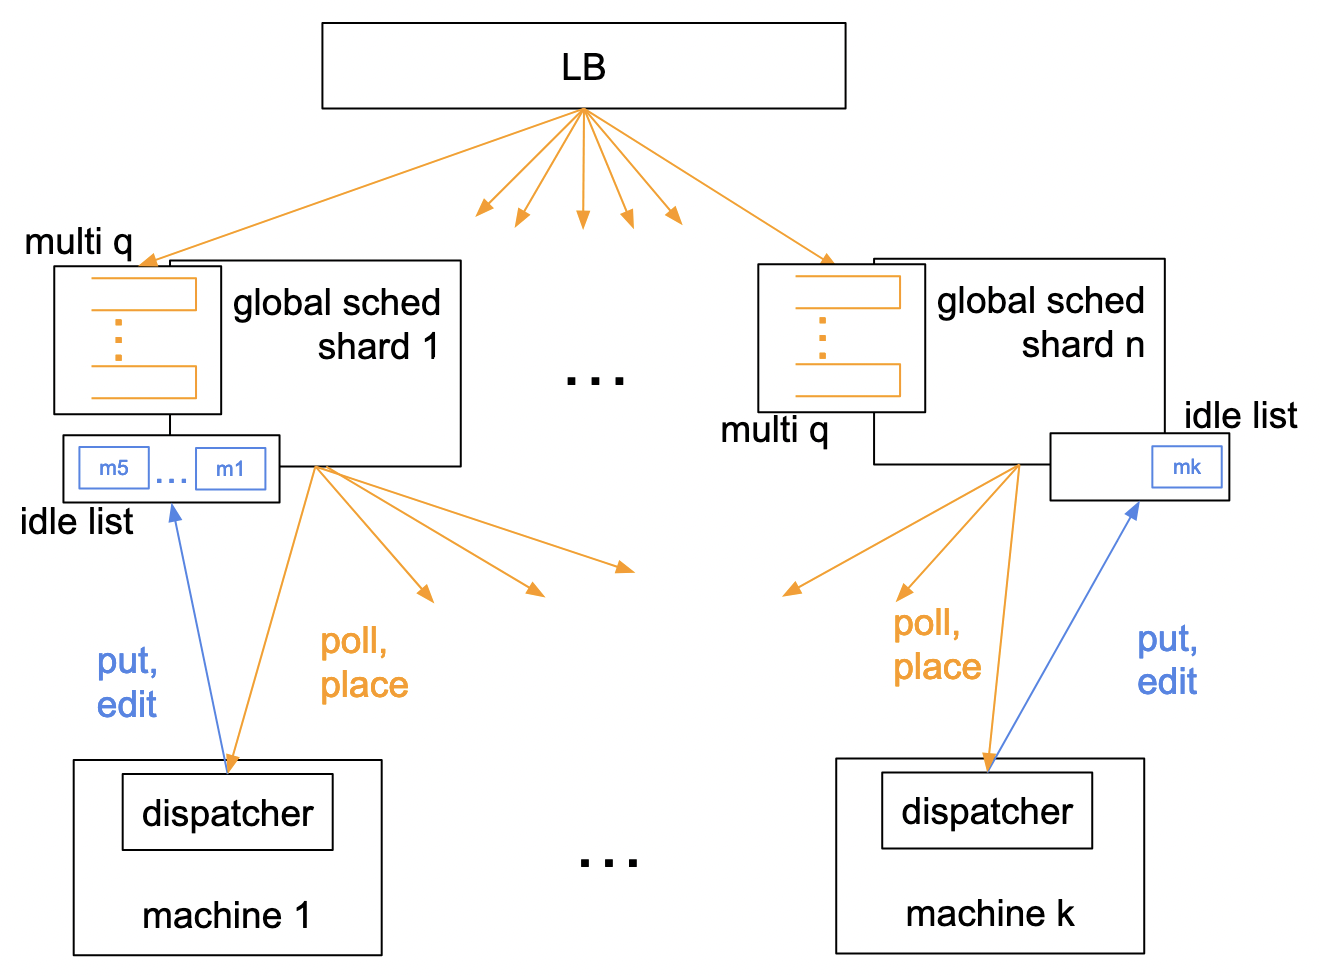
\includegraphics[width=8.5cm]{img/overview.png}
      \caption{ global scheduler shards queue and place functions (in orange),
      on each machine a dispatcher thread keeps track of memory utilization and
      writes itself to idle lists (in blue) }
    \label{fig:overview}
\end{figure}



\Sys{} has as its goal to enforce the \class{}es attached to
functions, which means it needs to prefer higher \class{} functions
over lower ones, and preempt the latter when necessary. As shown in
Figure~\ref{fig:overview}, \sys{} sits behind a load balancer, and
consists of: a \textit{distributed global scheduler}, which places new
function invocations and has attached an \textit{idle list}, a
\textit{dispatcher}, which runs on each machine and communicates with
the global scheduler shards, and a \textit{machine scheduler}, which
enforces \class{}es on the machines.


\textbf{Machine Scheduler.}
The machine scheduler is a preemptive priority scheduler: it preempts lower
\class{} functions to run higher \class{} ones. Being unfair and starving low
\class{} functions is desirable in \sys{}, since image processing functions
should not interrupt a page view request processing, but vice versa is expected.
Within \class{}es the machine scheduler is first come first served. This design
matches Linux' ``SCHED FIFO'' policy~\cite{linux-sched}.


\textbf{Idle list.}  Each global scheduler shard has an idle list,
which holds machines that have a significant amount of memory
available. In the shards idle list, each machine's entry is associated
with the amount of memory available as well as the current amount of
functions on the machine. The idle list exists because datacenters are
large: polling a small number of machines cannot find something that
is a rare occurrence~\cite{join-idle-queue}. The idle list allows the
rare idle machine to make itself visible to the global scheduler. The
idle list also allows the global scheduler to place high \class{}
functions quickly, without incurring the latency overheads of doing
polling to find available resources. This design is inspired by Join
Idle Queue~\cite{join-idle-queue}, but defines idleness via memory
availability rather than empty queues.


\textbf{Dispatcher.}
The dispatcher is in charge of adding itself to a shard's idle list when memory
utilization is low. The dispatcher chooses which list to add itself to using
power-of-$k$-choices: it looks at $k$ shards' idle lists and chooses the one with
the least other machines in it. If the machine is already on shard $i$'s idle
list, but the amount of available memory has changed significantly (either by
functions finishing and memory being freed or by memory utilization increasing
because of new functions or memory antagonists), the dispatcher will update
shard $i$'s idle list.

The dispatcher is also in charge of managing the machine's memory. When memory
pressure occurs, the dispatcher uses \textit{\class{}-based swapping} to move
low \class{} functions off the machine's memory. Having prices classes
creates an opportunity: because the dispatcher knows that the lowest \class{}
functions will not be run until the high \class{} functions have all finished,
it can swap its memory out knowing it will not be needed soon. The dispatcher
swaps the low \class{} function back in when the memory pressure is gone and the
function will be run.

\Sys{} cannot bound the amount of swap space required since it doesn't ask
functions for a memory bound.  In the rare case that memory still runs out,
\sys{} resorts to killing low \class{} functions.  Providers can estimate the
amount of swap space required by looking at memory utilization, and since the
SSDs necessary for swap space are inexpensive~\cite{ssd-price} we expect that
killing is rare.

\textbf{Global Scheduler Shards.}
Global scheduler shards store the functions waiting to be placed in a multi
queue, with one queue per \priceclass{}. Shards choose what function to place
next by looking at each function at the head of each queue, and comparing the
ratio of \class{} to amount of time spent in the queue. This policy ensures
that high \class{} functions don't have to wait as long as low \class{}
functions to be chosen next, but low \class{} functions will get placed if they
have waited for a while.

When placing the chosen function, the shard will first look in its
idle list. If the list is not empty, it will choose the machine with
the smallest queue length.  If there are no machines in the idle list,
the shard switches to power-of-$k$-choices: it polls $k$ machines, and
chooses the least loaded machine (by number of functions running).

%-------------------------------------------------------------------------------
\section{Current State}
%-------------------------------------------------------------------------------

Implementing this design required changing linux's EEVDF implementation. Linux's
EEVDF scheduler has a strong tenant of avoiding unfairness, and as a result
implements eligibility solely as a function of how much time a process had
gotten compared to other processes. This means that (assuming equally weighted
processes), after a tick of running, a process becomes ineligible, because it
got more time that it should have (in an ideal system the tick would have been
shared equally among all processes).

In \sysname, however, being able to be unfair for long periods of time is key:
jobs with short deadlines need to get absolute priority over jobs that have
later deadlines. To achieve this goal we had to modify Linux's EEVDF
implementation, to include the notion of request-based eligibility.

We developed a prototype application that follows the scheme of the website:
four different types of jobs, with deadlines ranging from 15ms to 6s, and
maximum computes from 12ms to 4s. Figure~\ref{fig:graph} shows the results on a
single machine, with and without the change to linux. 

Overall the graph shows success: being temporarily unfair to longer processes
that had a large amount of slack allowed the shorter processes with less slack
to consistently complete on time.
\section{Related work}

Some existing work focuses on isolating real-time applications in
Linux~\cite{rt-in-linux, state-rt-linux}, while Wasted Cores~\cite{wasted-cores}
focuses on the idle behavior of the Linux scheduler.

Other systems work around the kernel scheduler, by running primarily in
userspace~\cite{perfiso,caladan,skyloft}.

Linux's own \schedidle{} policy attempts to address this issue, but does not
fully solve it (running the microbenchmark using \schedidle{} still leads to an
increase in the mean latency from 6ms to 8).

%-------------------------------------------------------------------------------
% \bibliography{paper.bib}
\printbibliography

%%%%%%%%%%%%%%%%%%%%%%%%%%%%%%%%%%%%%%%%%%%%%%%%%%%%%%%%%%%%%%%%%%%%%%%%%%%%%%%%
\end{document}
%%%%%%%%%%%%%%%%%%%%%%%%%%%%%%%%%%%%%%%%%%%%%%%%%%%%%%%%%%%%%%%%%%%%%%%%%%%%%%%%

%%  LocalWords:  endnotes includegraphics fread ptr nobj noindent
%%  LocalWords:  pdflatex acks
